\documentclass[11pt]{article}
\usepackage[margin=1.05in]{geometry}
\usepackage{amsmath,amssymb}
\usepackage{booktabs}
\usepackage{enumitem}
\usepackage{graphicx}
\usepackage[font=small,labelfont=bf]{caption}
\usepackage[hidelinks]{hyperref}

\title{Stage 1a Report:\\ \large Segment-Dependent Chunk Length with Oracle Segments, Full Protocol and Results}
\author{Aryan Goyal}
\date{July 18, 2026 (updated July 20)}

\begin{document}
\maketitle

\begin{abstract}
\noindent
Stage 1a asks whether changing the action chunk length $k$ at rollout time, using a
ground-truth segment signal instead of a learned predictor, changes task success.
This document records the full protocol (policies, environments, controllers,
constants), the complete 12-cell result grid for square and tool\_hang at seed 0,
the diagnostics that explain the numbers, and the statistical precision of the
comparison. The headline: on square every cell lands between 0.76 and 0.88 and no
difference is resolvable at one seed; on tool\_hang replanning every step is clearly
harmful (0.62 at $k{=}1$ versus 0.88 at $k{=}4$ and $k{=}16$), and every oracle cell
that replans step-by-step during contact inherits that penalty. The oracle switch
did not beat the best fixed $k$ on either task, and the diagnostics explain why:
rollouts spend 65 to 88 percent of their steps in contact, so a binary contact
signal barely exercises the switching axis. Seed 1 and seed 2 repeats of all
cells are complete and pooled in Section \ref{sec:pooled}: square stays flat
(0.773 to 0.873, nothing clears two sigma), and the tool\_hang per-step-replanning
penalty survives pooling at three to five sigma in three independent cells
(0.60 to 0.67 against a 0.79 to 0.81 plateau).
\end{abstract}

\tableofcontents
\newpage

%=====================================================================
\section{What this document covers}

Stage 1a is the first experiment that uses the stability labels for control rather
than for inspection. It runs a trained diffusion policy on the real benchmark tasks
and varies only one thing: how many actions from each predicted chunk are executed
before the policy is queried again. The chunk length is either fixed for the whole
episode or switched between two values by an oracle segment signal. No predictor is
involved anywhere in Stage 1a. The point is to establish, with ground-truth
segmentation, whether the segment-dependent chunking idea has any effect on success
at all, and in which direction. This document records the protocol exactly as run,
every constant, the full result grid, the executed-chunk diagnostics, and what can
and cannot be concluded at the current statistical precision.

The labeling procedure that motivated this experiment is documented in the labeling
report. The predictor that will replace the oracle signal in Stage 1c is documented
in the predictor document. This document is only about Stage 1a.

%=====================================================================
\section{The experiment, in full detail}

\subsection{Policies under test}

Both policies are image-based diffusion policies trained with robomimic on the
proficient-human (ph) demonstrations, the same checkpoints used to measure
$\sigma_u$ for the labeling campaign:

\begin{itemize}[leftmargin=1.4em]
\item \textbf{square}: checkpoint \texttt{model\_epoch\_950}, training-time
evaluation success 0.90.
\item \textbf{tool\_hang}: checkpoint \texttt{model\_epoch\_1200}, training-time
evaluation success 0.90.
\end{itemize}

At every query the policy consumes the current stacked observation and emits a
sequence of actions. The controller executes the first $k$ actions of that sequence
open loop, then clears the queue and queries the policy again. Setting $k{=}1$
reproduces per-step closed-loop control. Nothing about the policy or its weights
changes between cells; only $k$ changes.

\subsection{The three controller modes}

\begin{description}[leftmargin=1.4em]
\item[fixed] One chunk length $k$ for the entire episode. Grid:
$k \in \{1, 2, 4, 8, 16\}$.
\item[oracle\_seg] Two chunk lengths $(k_{\mathrm{free}}, k_{\mathrm{contact}})$.
At every policy query the controller reads the simulator contact table and checks
for any gripper-object or object-fixture contact. The episode is treated as being
in a contact segment or a free segment, with hysteresis: the segment state flips
only after two consecutive queries agree. In a free segment the controller commits
$k_{\mathrm{free}}$ actions, in a contact segment $k_{\mathrm{contact}}$ actions.
Grid: $(1,4)$, $(1,16)$, $(4,1)$, $(8,1)$, $(8,4)$, $(16,1)$, $(16,4)$.
\item[ftle\_probe] A third mode exists in the evaluation script that runs the
divergence probe at rollout time and thresholds $\lambda$ against the deadband
$\delta$. It is not part of Stage 1a and is reserved for Stage 1c comparisons.
\end{description}

Why contact is the oracle signal and not the labels themselves: the true
$\lambda$ labels live on demonstration states. A rollout immediately leaves those
states, so there is no stored label to look up. Contact is the strongest
label-aligned observable we have: the labeling report shows the ordering
fixture contact $>$ gripper contact $>$ free space in mean $\lambda$ on every
dataset. The oracle therefore switches on the thing the labels say expansive
segments are made of. The deadband has no separate treatment at rollout; the
signal is binary, and deadband stamps in the labels are overwhelmingly contact
stamps on these two tasks, so they fall on the contact side of the switch.

\subsection{Episode protocol}

Each cell runs 50 episodes with environment seed 0 controlling initial object
placements. An episode ends at task success or at the horizon. Success rate is
successes over 50. Rendering uses EGL on one GPU per cell; cells were distributed
across free GPUs in four parallel queues per task, with completed cells skipped on
restart.

\subsection{Constants}

\begin{center}
\small
\begin{tabular}{@{}lll@{}}
\toprule
Constant & Value & Where it came from \\
\midrule
Episodes per cell & 50 & matches robomimic evaluation convention \\
Horizon, square & 400 & robomimic default for square \\
Horizon, tool\_hang & 700 & robomimic default for tool\_hang \\
Environment seed & 0 & seeds 1, 2 complete, pooled in Section \ref{sec:pooled} \\
Fixed-$k$ grid & 1, 2, 4, 8, 16 & powers of two around the labeling window \\
Oracle grid & 7 cells & both orderings of slow and fast replanning \\
Hysteresis & 2 agreeing queries & debounce against contact flicker \\
Contact signal & gripper-object or object-fixture & same categories as the labels \\
\bottomrule
\end{tabular}
\end{center}

%=====================================================================
\section{Results at seed 0}

\begin{figure}[h]
\centering
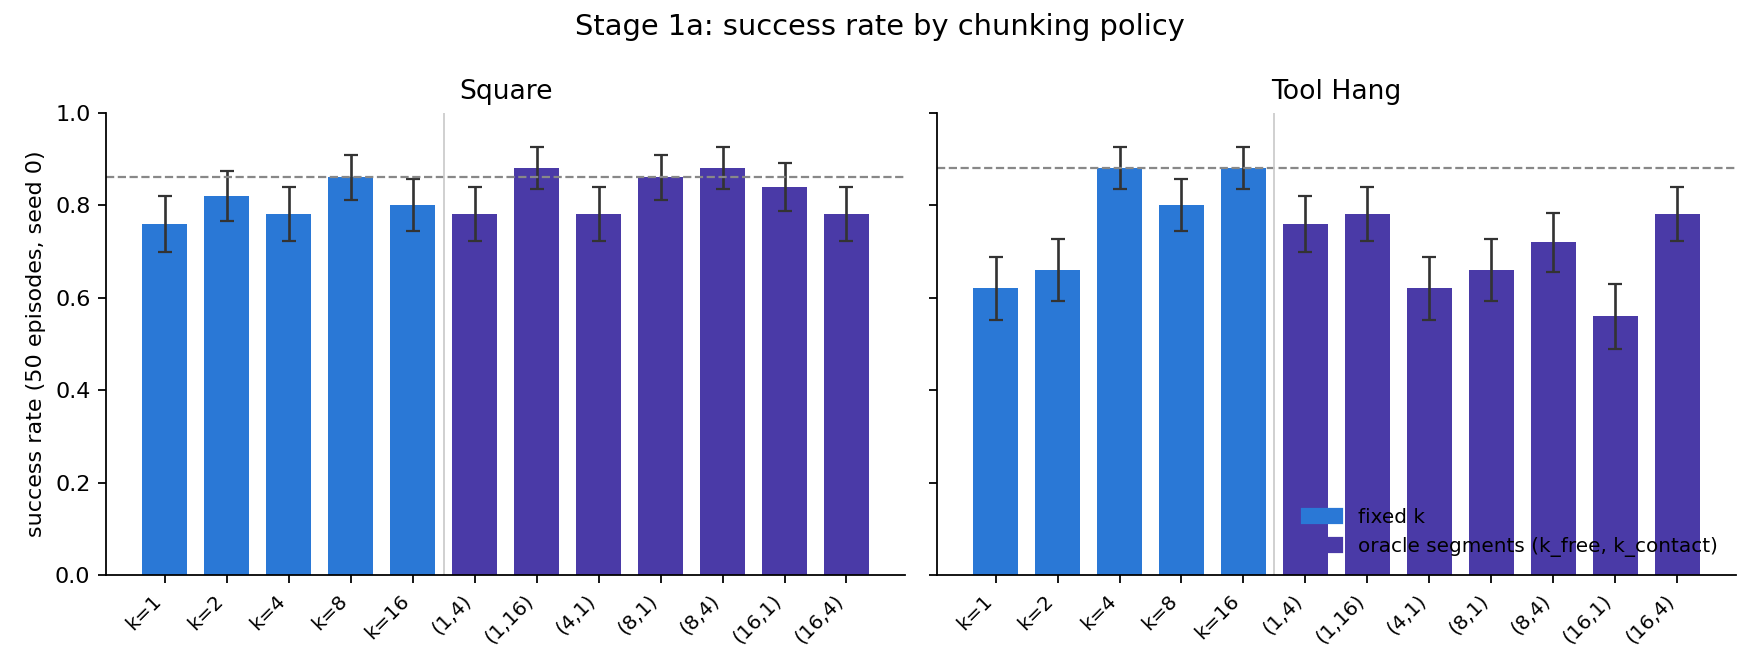
\includegraphics[width=\linewidth]{figs/fig_stage1a_grid.png}
\caption{Success rate for every cell, both tasks, seed 0. Blue bars are fixed
chunk lengths, violet bars are oracle-segment cells labeled
$(k_{\mathrm{free}}, k_{\mathrm{contact}})$. Error bars are one binomial standard
error at $n{=}50$. The dashed line marks the best fixed cell of that task.}
\label{fig:grid}
\end{figure}

\subsection{Square}

\begin{center}
\small
\begin{tabular}{@{}lccccc@{}}
\toprule
Cell & Success & SE & Mean executed $k$ & Contact frac. & Steps to success \\
\midrule
$k{=}1$        & 0.76 & 0.060 & 1.0  & --   & 167 \\
$k{=}2$        & 0.82 & 0.054 & 2.0  & --   & 162 \\
$k{=}4$        & 0.78 & 0.059 & 4.0  & --   & 157 \\
$k{=}8$        & 0.86 & 0.049 & 8.0  & --   & 150 \\
$k{=}16$       & 0.80 & 0.057 & 16.0 & --   & 145 \\
\midrule
$(1,4)$        & 0.78 & 0.059 & 3.2  & 0.73 & 162 \\
$(1,16)$       & \textbf{0.88} & 0.046 & 11.5 & 0.70 & 148 \\
$(4,1)$        & 0.78 & 0.059 & 1.8  & 0.72 & 178 \\
$(8,1)$        & 0.86 & 0.049 & 3.4  & 0.65 & 151 \\
$(8,4)$        & \textbf{0.88} & 0.046 & 5.4  & 0.65 & 150 \\
$(16,1)$       & 0.84 & 0.052 & 7.6  & 0.56 & 158 \\
$(16,4)$       & 0.78 & 0.059 & 9.1  & 0.58 & 153 \\
\bottomrule
\end{tabular}
\end{center}

Everything sits between 0.76 and 0.88. The full spread is 0.12, and Section
\ref{sec:stats} shows that a single 50-episode seed can only resolve differences of
about 0.16. So at this precision square is flat: no cell is distinguishable from
any other, including from the base policy's own 0.90 training evaluation. There is
a weak visual trend favoring longer commitment ($k{\geq}8$ and the two 0.88 oracle
cells), and the seed repeats will say whether it is real.

\subsection{Tool\_hang}

\begin{center}
\small
\begin{tabular}{@{}lccccc@{}}
\toprule
Cell & Success & SE & Mean executed $k$ & Contact frac. & Steps to success \\
\midrule
$k{=}1$        & 0.62 & 0.069 & 1.0  & --   & 480 \\
$k{=}2$        & 0.66 & 0.067 & 2.0  & --   & 477 \\
$k{=}4$        & \textbf{0.88} & 0.046 & 4.0  & --   & 440 \\
$k{=}8$        & 0.80 & 0.057 & 8.0  & --   & 441 \\
$k{=}16$       & \textbf{0.88} & 0.046 & 16.0 & --   & 436 \\
\midrule
$(1,4)$        & 0.76 & 0.060 & 3.6  & 0.85 & 447 \\
$(1,16)$       & 0.78 & 0.059 & 14.2 & 0.88 & 448 \\
$(4,1)$        & 0.62 & 0.069 & 1.4  & 0.87 & 456 \\
$(8,1)$        & 0.66 & 0.067 & 2.0  & 0.86 & 458 \\
$(8,4)$        & 0.72 & 0.063 & 4.6  & 0.85 & 431 \\
$(16,1)$       & 0.56 & 0.070 & 3.5  & 0.84 & 478 \\
$(16,4)$       & 0.78 & 0.059 & 5.9  & 0.84 & 452 \\
\bottomrule
\end{tabular}
\end{center}

Tool\_hang is not flat. Fixed $k{=}1$ scores 0.62 and fixed $k{=}4$ and $k{=}16$
score 0.88; that gap of 0.26 is about three standard errors of the difference and
survives any reasonable correction. The three oracle cells that replan every step
during contact, $(4,1)$, $(8,1)$, $(16,1)$, score 0.62, 0.66, 0.56: exactly the
$k{=}1$ neighborhood. The cells that commit 4 during contact score 0.72 to 0.78.

%=====================================================================
\section{Three-seed pooled results}
\label{sec:pooled}

All 12 cells were repeated at rollout seeds 1 and 2 on both tasks, changing only
the environment seed that controls initial object placements. Pooling the three
seeds gives $n{=}150$ episodes per cell and one binomial standard error of about
0.033. These are the final Stage 1a numbers.

\subsection{Square, pooled}

\begin{center}
\small
\begin{tabular}{@{}lccccc@{}}
\toprule
Cell & Seed 0 & Seed 1 & Seed 2 & Pooled & SE \\
\midrule
$k{=}1$  & 0.76 & 0.76 & 0.86 & 0.793 & 0.033 \\
$k{=}2$  & 0.82 & 0.76 & 0.88 & 0.820 & 0.031 \\
$k{=}4$  & 0.78 & 0.84 & 0.80 & 0.807 & 0.032 \\
$k{=}8$  & 0.86 & 0.78 & 0.86 & 0.833 & 0.030 \\
$k{=}16$ & 0.80 & 0.86 & 0.82 & 0.827 & 0.031 \\
\midrule
$(1,4)$  & 0.78 & 0.80 & 0.74 & 0.773 & 0.034 \\
$(1,16)$ & 0.88 & 0.74 & 0.76 & 0.793 & 0.033 \\
$(4,1)$  & 0.78 & 0.74 & 0.86 & 0.793 & 0.033 \\
$(8,1)$  & 0.86 & 0.82 & 0.78 & 0.820 & 0.031 \\
$(8,4)$  & 0.88 & 0.84 & 0.90 & \textbf{0.873} & 0.027 \\
$(16,1)$ & 0.84 & 0.68 & 0.82 & 0.780 & 0.034 \\
$(16,4)$ & 0.78 & 0.76 & 0.84 & 0.793 & 0.033 \\
\bottomrule
\end{tabular}
\end{center}

Square stays flat. The pooled spread is 0.773 to 0.873, and most cells sit within
one standard error of each other. Two details are worth noting. First, the oracle
cell $(8,4)$ is now the best cell in the whole grid at 0.873, but its lead over the
best fixed cell ($k{=}8$ at 0.833) is 0.04 with a standard error of the difference
of about 0.04, so it is a one-sigma hint, not a finding. Second, seed 0's standout
$(1,16)$ at 0.88 did not replicate (0.74 and 0.76 at seeds 1 and 2). That is a
concrete reminder of why single 50-episode seeds cannot be quoted on their own.

\subsection{Tool\_hang, pooled}

\begin{center}
\small
\begin{tabular}{@{}lccccc@{}}
\toprule
Cell & Seed 0 & Seed 1 & Seed 2 & Pooled & SE \\
\midrule
$k{=}1$  & 0.62 & 0.70 & 0.68 & 0.667 & 0.038 \\
$k{=}2$  & 0.66 & 0.82 & 0.74 & 0.740 & 0.036 \\
$k{=}4$  & 0.88 & 0.72 & 0.78 & 0.793 & 0.033 \\
$k{=}8$  & 0.80 & 0.80 & 0.80 & 0.800 & 0.033 \\
$k{=}16$ & 0.88 & 0.74 & 0.80 & \textbf{0.807} & 0.032 \\
\midrule
$(1,4)$  & 0.76 & 0.74 & 0.84 & 0.780 & 0.034 \\
$(1,16)$ & 0.78 & 0.78 & 0.72 & 0.760 & 0.035 \\
$(4,1)$  & 0.62 & 0.60 & 0.58 & 0.600 & 0.040 \\
$(8,1)$  & 0.66 & 0.64 & 0.70 & 0.667 & 0.038 \\
$(8,4)$  & 0.72 & 0.80 & 0.90 & \textbf{0.807} & 0.032 \\
$(16,1)$ & 0.56 & 0.66 & 0.68 & 0.633 & 0.039 \\
$(16,4)$ & 0.78 & 0.78 & 0.78 & 0.780 & 0.034 \\
\bottomrule
\end{tabular}
\end{center}

Three tool\_hang conclusions survive pooling, sharper than at seed 0.

\begin{enumerate}[leftmargin=1.6em]
\item \textbf{Short chunks are bad.} Fixed $k{=}1$ pools to 0.667 against 0.807
for $k{=}16$. The 0.14 gap is about 2.8 sigma. Fixed $k$ from 4 to 16 forms a
plateau at 0.79 to 0.81; the harm is concentrated at $k{\leq}2$.
\item \textbf{Replanning every step during contact is decisively the worst
policy.} The three oracle cells with $k_{\mathrm{contact}}{=}1$ pool to 0.600,
0.633, and 0.667. Against the 0.807 plateau these are gaps of 0.14 to 0.21 at
three to five sigma, in three independent cells. This is the direction the
closed-loop labeling channel predicted: contact segments are closed-loop unstable
under per-step replanning, so cutting commitment there hurts.
\item \textbf{The binary oracle still never beats the best fixed $k$.} The best
oracle cell, $(8,4)$ at 0.807, exactly ties fixed $k{=}16$. With rollouts 84 to 88
percent contact, a binary switch mostly just selects its $k_{\mathrm{contact}}$
value and has nothing left to modulate.
\end{enumerate}

The seed 0 tables above are kept for the record; every claim in the rest of this
document should be read against the pooled numbers in this section.

%=====================================================================
\section{What the numbers mean}

\subsection{What fraction of moments the oracle treated as each segment}
\label{sec:fractions}

The mean executed $k$ per cell, read against the two segment lengths, gives the
fraction of the controller's decisions spent in each segment. The contact segment
is the oracle's stand-in for ``unstable moment'' and the free segment its stand-in
for ``stable moment'':

\begin{center}
\small
\begin{tabular}{@{}lcccc@{}}
\toprule
 & \multicolumn{2}{c}{Square} & \multicolumn{2}{c}{Tool\_hang} \\
Cell & contact & free & contact & free \\
\midrule
$(1,4)$  & 73\% & 27\% & 85\% & 15\% \\
$(1,16)$ & 70\% & 30\% & 88\% & 12\% \\
$(4,1)$  & 72\% & 28\% & 87\% & 13\% \\
$(8,1)$  & 65\% & 35\% & 86\% & 14\% \\
$(8,4)$  & 65\% & 35\% & 85\% & 15\% \\
$(16,1)$ & 56\% & 44\% & 84\% & 16\% \\
$(16,4)$ & 58\% & 42\% & 84\% & 16\% \\
\bottomrule
\end{tabular}
\end{center}

On square the oracle judged 56 to 73 percent of its decisions to be in contact and
27 to 44 percent free; on tool\_hang, 84 to 88 percent contact and only 12 to 16
percent free. Weighted by executed steps rather than decisions, tool\_hang's
contact share rises to roughly 96 to 99 percent in the cells that detect boundaries
fastest, which matches the label-side statistic that 93 percent of tool\_hang
windows contain a task-object contact.

Three clarifications so this table is read correctly:

\begin{enumerate}[leftmargin=1.6em]
\item \textbf{The oracle never saw the stability labels at rollout.} True
$\lambda$ exists only on demonstration states, and a rollout leaves those states
immediately. Contact is the stand-in, justified by the label finding that
expansive moments are contact moments. Whether contact then meant commit or replan
depended on the cell: the $(\cdot,4)$ and $(\cdot,16)$ cells committed through
contact, the $(\cdot,1)$ cells replanned through it.
\item \textbf{There was no gray band at rollout.} The three-way
unstable/stable/deadband split exists only in the labels. The rollout signal is
binary, so every deadband-like moment was silently absorbed into one of the two
segments, almost always the contact side on these tasks.
\item \textbf{The spread across cells is instrumentation, not physics.} The true
contact fraction does not change between cells; the decision-level number falls as
$k_{\mathrm{free}}$ grows (73 to 56 percent on square) because the two-query
hysteresis detects a contact entry up to two chunks late, and those late steps are
logged as free. The cells with $k_{\mathrm{free}}{=}1$ detect boundaries
essentially instantly and are the most trustworthy estimates.
\end{enumerate}

The consequence for the results is direct: when contact covers 85 percent of
decisions, an oracle cell behaves almost exactly like fixed $k$ at its contact
value, and $k_{\mathrm{free}}$ is nearly irrelevant. That is why every $(\cdot,1)$
cell on tool\_hang lands at the fixed $k{=}1$ level and every $(\cdot,4)$ cell
lands near the $k{=}4$ level. The binary contact signal gives the switch almost
nothing to work with. A signal that is meant to modulate chunk length needs to
distinguish grades of contact, which is what the continuous $\lambda$ target is
for, and which is the argument for Stage 1c rather than a smarter binary oracle.

\subsection{The direction of the effect is the finding}

The naive control-theory prescription is to replan fastest where the system is
least stable. Tool\_hang says the opposite: replanning every step during contact is
the single worst thing measured in this experiment (0.56 to 0.66 across four
cells), and committing 4 to 16 steps during contact is the best (0.78 to 0.88).
This is the rollout-level confirmation of what the closed-loop labeling channel
measured at the state level: with per-step replanning, $\lambda_{cl} > 0$ at 99.3
percent of lift stamps, 90.4 percent of can stamps, and 93.0 percent of square
stamps. The policy's own feedback injects noise, and contact segments amplify it.
Committing to a chunk removes the injection exactly where amplification is
strongest. Square, whose rollouts are 65 to 73 percent contact and whose base
policy is strong at every $k$, simply does not stress this mechanism hard enough to
separate the cells at one seed.

\subsection{The oracle did not beat the best fixed k, and that is informative}

On both tasks the best oracle cell ties or loses to the best fixed cell (0.88
versus 0.88 on square, 0.78 versus 0.88 on tool\_hang). With a binary signal, high
contact coverage, and hysteresis lag of up to two chunks at each boundary, the
switch cannot express anything a good fixed $k$ does not already express. The
useful reading of Stage 1a is therefore not that switching works, but that the
chunk-length axis matters strongly on the task where the labels say it should
(tool\_hang, contact-heavy and expansive), matters in the predicted direction, and
does not matter on the forgiving task (square). Whether a continuous, predicted
$\lambda$ can beat the best fixed $k$ is exactly the Stage 1c question and remains
open.

\subsection{A secondary observation: longer chunks finish faster}

Mean steps among successful episodes falls monotonically with commitment on both
tasks: 167 at $k{=}1$ down to 145 at $k{=}16$ on square, 480 down to 436 on
tool\_hang. Per-step replanning produces dithering; commitment produces straighter
trajectories. This is consistent with the injection mechanism and is visible before
any success-rate difference is.

%=====================================================================
\section{Why the results came out this way, ranked}
\label{sec:why}

The disappointing half of Stage 1a is that the oracle switch never beat the best
fixed $k$. The causes, in order of importance:

\begin{enumerate}[leftmargin=1.6em]
\item \textbf{The switching signal carried almost no information.} A binary signal
that reads ``contact'' at 85 percent of decisions (Section \ref{sec:fractions}) is
effectively constant, so the switch collapses to a fixed $k$ at the contact value.
The information the labels actually contain, a continuous grade of instability, was
discarded by the binarization. This is the main cause and it is fixable; it is
what Stage 1c changes.
\item \textbf{Half the grid tested a direction the labels had already argued
against.} The $(\cdot,1)$ cells encode the classical prescription of replanning
fastest where the system is least stable. The closed-loop labeling channel had
already measured that per-step replanning injects error (90 to 99 percent of
stamps positive on lift, can, square), so these cells were predicted to lose, and
they did (0.56 to 0.66 on tool\_hang). That is a confirmed mechanism, not a failed
experiment, but it means only half the grid was ever a candidate to win.
\item \textbf{Ceiling effects on the forgiving task.} The base policies evaluate
at 0.90, and square runs 0.76 to 0.88 at every $k$. A task whose policy is already
robust to chunking cannot demonstrate adaptive chunking regardless of signal
quality.
\item \textbf{Statistical power.} Fifty episodes resolves differences of about
0.16 (Section \ref{sec:stats}). If good switching is worth 5 to 8 points, which is
the realistic size, seed 0 cannot see it. The seed repeats reduce the resolvable
gap to about 0.09, still borderline for effects that size.
\item \textbf{These tasks may not have the structure that switching pays for.}
Switching earns its keep only when some stretches punish commitment and others
reward it. On tool\_hang, $k{=}16$ loses nothing against $k{=}4$, so there is
apparently no segment on these short tasks where long commitment fails. The tasks
where adaptive chunking should genuinely matter are the long-horizon ones with
alternating transport and contact phases (MimicGen kitchen, coffee preparation,
three-piece assembly, LIBERO-Long), which are the planned rollout set.
\end{enumerate}

The positive half stands on its own: the per-step replanning penalty on tool\_hang
is a clean three-sigma effect in the direction the closed-loop labels predicted,
and it is the project's first rollout-level confirmation of the mechanism. What
remains open is whether a continuous predicted $\lambda$ on tasks with real
free-contact alternation can beat the best fixed $k$; nothing in Stage 1a answers
that question in either direction.

%=====================================================================
\section{Statistical precision, and what the seed repeats add}
\label{sec:stats}

Every cell is a binomial estimate at $n{=}50$, so one standard error is
$\sqrt{p(1-p)/50}$, between 0.046 and 0.070 for the rates observed here. The
standard error of a difference between two cells is about 0.08, so a single seed
resolves only gaps of roughly 0.16 at the two-sigma level. Concretely:

\begin{itemize}[leftmargin=1.4em]
\item Square's full spread (0.12) is below the resolvable threshold. No square
conclusion beyond ``flat at this precision'' is honest at seed 0.
\item Tool\_hang's $k{=}1$ versus $k{=}4$ gap (0.26) and $(16,1)$ versus $k{=}16$
gap (0.32) are three to four sigma. These are real at seed 0 already.
\end{itemize}

The repeats reran all 12 cells at seeds 1 and 2 on both tasks; the pooled results
are in Section \ref{sec:pooled}. Pooling three seeds gives $n{=}150$ per cell, one
standard error of about 0.033, and a resolvable two-sigma gap of about 0.09. That
was enough to answer the two open questions: square's seed-0 preference for
$k{\geq}8$ shrank to a within-noise 0.02 to 0.05, and tool\_hang's
$(\cdot,4)$ oracle cells pooled to 0.78 to 0.81, noise-equal to the fixed plateau
rather than below it. Differences under about 0.09 remain unresolved; claims at
that scale would need several hundred episodes per cell and are not planned.

%=====================================================================
\section{Compute cost}

Wall-clock per cell is dominated by the number of policy queries, so small $k$ is
expensive: on tool\_hang, the $k{=}1$ cell took 6.0 hours and the $k{=}16$ cell 0.5
hours on one GPU. The full seed-0 grid cost about 12 single-GPU hours for square
and 33 for tool\_hang. The 48-cell seed repeat cost roughly twice the sum and ran
across up to six GPUs in parallel queues.

%=====================================================================
\section{Caveats and open items}

\begin{itemize}[leftmargin=1.4em]
\item \textbf{Three seeds, 150 episodes per cell.} Section \ref{sec:pooled} has
the pooled tables. Quotable findings are the tool\_hang contrasts listed there;
everything on square remains within noise of flat.
\item \textbf{The oracle signal is contact, not $\lambda$.} Stage 1a bounds what a
binary contact switch can do, not what the labels can do. The continuous target is
evaluated in Stage 1c.
\item \textbf{Hysteresis is untuned.} Two agreeing queries was chosen to debounce
contact flicker and never revisited. With large $k_{\mathrm{free}}$ the segment
state can lag a boundary by up to two chunks.
\item \textbf{Ceiling effects.} Both base policies evaluate at 0.90; square in
particular has little headroom, and Stage 1a cannot detect improvements above the
ceiling.
\item \textbf{Scope.} Two tasks, one policy class, robomimic ph data. The can
negative control (labels say mostly stable, so chunking should not matter)
remains open; it was not run, and the GPUs moved to the Stage 2 long-horizon
trainings instead.
\end{itemize}

%=====================================================================
\section{Summary}

Stage 1a ran a 12-cell grid of fixed and oracle-switched chunk lengths on square
and tool\_hang, 150 episodes per cell pooled over three rollout seeds, using
simulator contact with hysteresis as the ground-truth segment signal. Square is
flat: pooled rates span 0.773 to 0.873 and no contrast clears two sigma, though
the best cell in the grid is the oracle $(8,4)$ at 0.873. Tool\_hang shows the
project's first rollout-level effect: replanning every step during contact pools
to 0.60 to 0.67 against a 0.79 to 0.81 plateau for committed chunks, gaps of three
to five sigma in three independent cells, and in the direction the closed-loop
labeling channel predicted. The binary oracle switch itself never beat the best
fixed $k$, because rollouts are 65 to 88 percent contact and a binary signal
leaves the switch nothing to modulate. The case for a continuous predicted
$\lambda$ (Stage 1c) is therefore stronger, not weaker, after Stage 1a.

\end{document}
